
\begin{comment}
\begin{table*}[!ht]
\centering
\resizebox{0.7\textwidth}{!}{%
\begin{tabular}{ | p{0.07\textwidth} |
                   p{0.54\textwidth} | p{0.55\textwidth} |
                 }
\toprule
\textbf{Prompt} &
  Will the next great writer be a robot? &
  AI-generated text is impossible to detect! 
   \\ \hline
\rotatebox[origin=r]{90}{\parbox[c]{5cm}{\centering \textbf{AI-generated hallucinated text}}} &
    {I'm \colorbox{pink}{very skeptical} that the next ``great writer'' is going to be a robot, \colorbox{pink}{or} that they'll be \colorbox{pink}{much} more effective at \colorbox{pink}{expressing the} subtleties and depths of \colorbox{pink}{human} thought than a human is. However, what is \colorbox{pink}{most} interesting is the role that the \colorbox{pink}{Internet could} play in bringing these ''robot'' writers into the public eye. If I could (and I'm \colorbox{pink}{very} excited by this possibility), I would pay a \colorbox{pink}{small monthly} fee to \colorbox{pink}{read well-written}...} &
 { AI-generated text can be challenging to detect, especially with the advancements in natural language processing and machine learning. However, it is not accurate to say that AI-generated text is impossible to detect. There are various techniques and tools available that can help in identifying AI-generated content. Researchers and developers are actively working on improving detection methods to keep up with the evolving capabilities of AI models. While it may be difficult to distinguish between human-written and AI-generated text in some cases, ongoing efforts are being made to enhance detection and maintain transparency in communication.}
   \\ \hline
\rotatebox[origin=r]{90}{\parbox[c]{5cm}{\centering \textbf{De-hallucinated text by replacing high-entropy words}}} &
    {I'm \colorbox{green}{somewhat} skeptical that the next ``great writer'' is going to be a robot, \colorbox{green}{given} that they'll be \colorbox{green}{far} more effective at \colorbox{green}{grasping deeper} subtleties and depths of philosophical thought than a robot is. However, what is \colorbox{green}{particularly} interesting is the role that the Internet \colorbox{green}{may} play in bringing new great writers into the public eye. If I did (and I'm \colorbox{green}{extremely} excited by this possibility), I would pay a \colorbox{green}{hefty subscription} fee to \colorbox{green}{publish  something}...} & 
{AI-generated text can be challenging to detect, especially with the advancements in natural language processing and machine learning. However, it is not accurate to say that AI-generated text is impossible to detect. There are various techniques and tools available that can help in identifying AI-generated content. Researchers and developers are actively working on improving detection methods to keep up with the evolving capabilities of AI models. While it may be difficult to distinguish between human-written and AI-generated text in some cases, ongoing efforts are being made to enhance detection and maintain transparency in communication. }
   \\ \bottomrule
\end{tabular}
}
\caption{De-hallucination example}
\label{tab:my-table}
\end{table*}
\end{comment}

% \begin{figure*}
%   \begin{minipage}[t]{.65\linewidth}
%     \centering
%     % \includegraphics{example-image-duck}%
%     \begin{figure}
% [!htbp]
    \centering
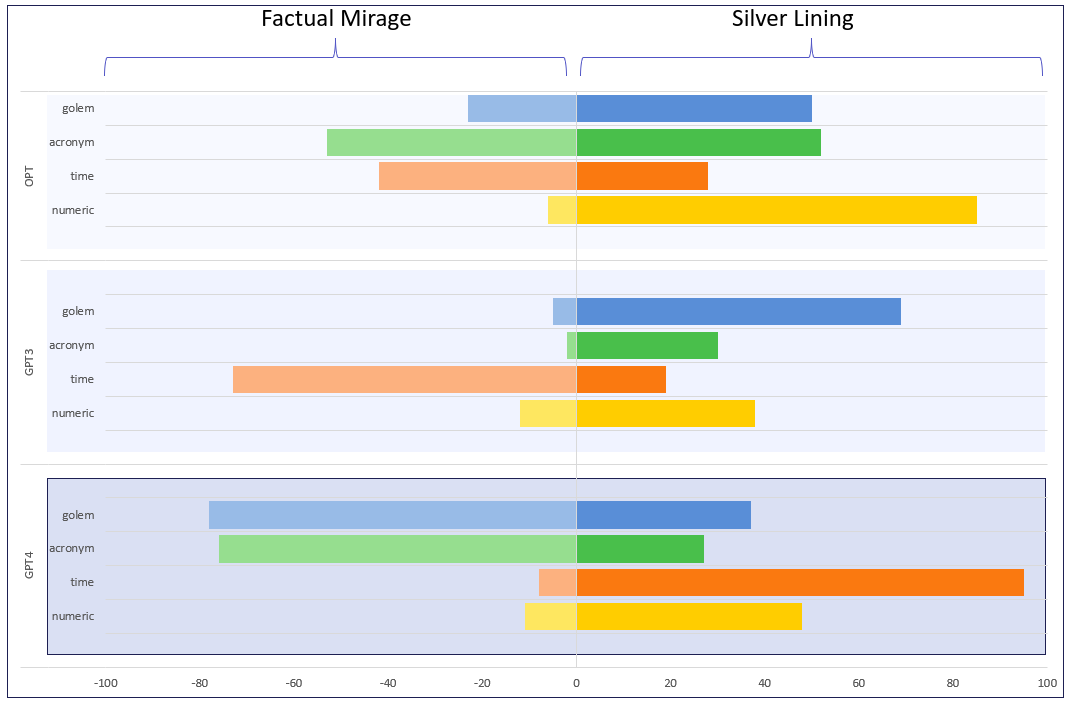
\includegraphics[width=\textwidth,height=9cm]{img/hvi.png}
    \caption{Hallucination Vulnerability Index \emph{(HVI)} for different hallucination categories for various LLMs \textcolor{red}{why does this figure have an arxiv link?}}
    \label{fig:hvi}
\end{figure}
%   \end{minipage}
%   % \hfill
%   \begin{minipage}[t]{.35\linewidth}
%     \centering
%     %\begin{table}[!ht]
%\tiny
%\centering
%\resizebox{0.32\textheight}{!}{%
\resizebox{0.9\columnwidth}{!}{%
\begin{tabular}{lll}
\toprule
\textbf{LLM} & \textbf{Size} & \textbf{HVI (0-100)}
\\ \midrule
\textbf{GPT-3}    &  175B       &   90 - 
\begin{tikzpicture}
\centering
\draw[red, very thick, fill=red] (0,0)  rectangle (5.62,.1);
\end{tikzpicture}
\\
\textbf{StableLM}    &  7B   &     82 - 
\begin{tikzpicture}
\centering
\draw[red, very thick, fill=red] (0,0)  rectangle (5.12,.1);
\end{tikzpicture}
\\
\textbf{GPT-2}    &   1.5B      &     70 - 
\begin{tikzpicture}
\centering
\draw[red, very thick, fill=red] (0,0)  rectangle (4.38,.1);
\end{tikzpicture}
\\
\textbf{Vicuna}     & 13B      &   62 - 
\begin{tikzpicture}
\centering
\draw[orange, very thick, fill=orange] (0,0)  rectangle (3.88,.1);
\end{tikzpicture}  
\\
\textbf{MPT}    &  7B    &     59 - 
\begin{tikzpicture}
\centering
\draw[orange, very thick, fill=orange] (0,0)  rectangle (3.69,.1);
\end{tikzpicture}   
\\
\textbf{LLaMA}    &  65B    &     57 - 
\begin{tikzpicture}
\centering
\draw[orange, very thick, fill=orange] (0,0)  rectangle (3.56,.1);
\end{tikzpicture}   
\\
\textbf{GPT-3.5}   &    175B      &     53 - 
\begin{tikzpicture}
\centering
\draw[orange, very thick, fill=orange] (0,0)  rectangle (3.31,.1);
\end{tikzpicture}
\\
\textbf{Dolly}    &   12B    &    49 - 
\begin{tikzpicture}
\centering
\draw[violet, very thick, fill=violet] (0,0)  rectangle (3.06,.1);
\end{tikzpicture} 
\\
\textbf{OPT}    &   175B   &     48 - 
\begin{tikzpicture}
\centering
\draw[violet, very thick, fill=violet] (0,0)  rectangle (3,.1);
\end{tikzpicture}   
\\
\textbf{GPT-4}    &   1.7T    &      47 - 
\begin{tikzpicture}
\centering
\draw[violet, very thick, fill=violet] (0,0)  rectangle (2.94,.1);
\end{tikzpicture}  
\\
\textbf{Alpaca}   &   65B    &     40 - 
\begin{tikzpicture}
\centering
\draw[violet, very thick, fill=violet] (0,0)  rectangle (2.5,.1);
\end{tikzpicture}   
\\
\textbf{BLOOM}   &   176B     &   38 - 
\begin{tikzpicture}
\centering
\draw[blue, very thick, fill=blue] (0,0)  rectangle (2.38,.1);
\end{tikzpicture}  
\\
\textbf{T0}    &      11B    &     36 - 
\begin{tikzpicture}
\centering
\draw[blue, very thick, fill=blue] (0,0)  rectangle (2.25,.1);
\end{tikzpicture}  
\\
\textbf{XLNet}   &   340M     &      36 - 
\begin{tikzpicture}
\centering
\draw[blue, very thick, fill=blue] (0,0)  rectangle (2.25,.1);
\end{tikzpicture}  
\\
\textbf{T5}    &    11B      &     32 - 
\begin{tikzpicture}
\centering
\draw[blue, very thick, fill=blue] (0,0)  rectangle (2.0,.1);
\end{tikzpicture}  
\\
% ERNIE           &     40 - \begin{tikzpicture}
% \centering
% \draw[violet, very thick, fill=violet] (0,0)  rectangle (2,.5);
% \end{tikzpicture}  
% \\
% ALBERT          &   33 - \begin{tikzpicture}
% \centering
% \draw[blue, very thick, fill=blue] (0,0)  rectangle (1.8,.5);
% \end{tikzpicture}    
% \\
% DeBERTa         &     32 - \begin{tikzpicture}
% \centering
% \draw[blue, very thick, fill=blue] (0,0)  rectangle (1.6,.5);
% \end{tikzpicture}    
% \\
% ELECTRA         &    32 - \begin{tikzpicture}
% \centering
% \draw[blue, very thick, fill=blue] (0,0)  rectangle (1.8,.5);
% \end{tikzpicture}     
% \\
% RoBERTa         &    28 - \begin{tikzpicture}
% \centering
% \draw[blue, very thick, fill=blue] (0,0)  rectangle (1.4,.5);
% \end{tikzpicture}     
% \\
% BERT            &    26 - \begin{tikzpicture}
% \centering
% \draw[blue, very thick, fill=blue] (0,0)  rectangle (1,.5);
% \end{tikzpicture}     
% \ \ 
\bottomrule
\end{tabular}%
}
%%
%}


%\caption{A ranked list of LLMs based on HVI.}
%\label{tab:LLMs}
%\end{table}
%\vspace{-3mm}









\begin{comment}
%\begin{table}[!ht]
%\tiny
%\centering
\resizebox{\columnwidth}{!}{%
\begin{tabular}{lll}
\toprule
\textbf{LLM} & \textbf{Size} & \textbf{HVI (0-100)}
\\ \midrule
\textbf{GPT 4}    &  N/A       &   90 - 
\begin{tikzpicture}
\centering
\draw[red, very thick, fill=red] (0,0)  rectangle (5,.1);
\end{tikzpicture}
\\
\textbf{GPT 3.5}    &  1.3B   &     82 - 
\begin{tikzpicture}
\centering
\draw[red, very thick, fill=red] (0,0)  rectangle (4.6,.1);
\end{tikzpicture}
\\
\textbf{GPT 3}     & 175B      &   70 - 
\begin{tikzpicture}
\centering
\draw[red, very thick, fill=red] (0,0)  rectangle (4.4,.1);
\end{tikzpicture}  
\\
\textbf{GPT 2}    &   1.5B    &      47 - 
\begin{tikzpicture}
\centering
\draw[red, very thick, fill=red] (0,0)  rectangle (4.2,.1);
\end{tikzpicture}  
\\
\textbf{MPT}   &    7B      &     59 - 
\begin{tikzpicture}
\centering
\draw[orange, very thick, fill=orange] (0,0)  rectangle (4.0,.1);
\end{tikzpicture}
\\
\textbf{OPT}    &   125M      &     59 - 
\begin{tikzpicture}
\centering
\draw[orange, very thick, fill=orange] (0,0)  rectangle (3.8,.1);
\end{tikzpicture}
\\
\textbf{LLaMA}    &   7B    &    52 - 
\begin{tikzpicture}
\centering
\draw[orange, very thick, fill=orange] (0,0)  rectangle (3.5,.1);
\end{tikzpicture} 
\\
\textbf{BLOOM}   &   175B     &   49 - 
\begin{tikzpicture}
\centering
\draw[orange, very thick, fill=orange] (0,0)  rectangle (3.3,.1);
\end{tikzpicture}  
\\
\textbf{Alpaca}    &   7B   &     44 - 
\begin{tikzpicture}
\centering
\draw[orange, very thick, fill=orange] (0,0)  rectangle (3.1,.1);
\end{tikzpicture}   
\\
\textbf{Vicuna}    &  7B    &     44 - 
\begin{tikzpicture}
\centering
\draw[violet, very thick, fill=violet] (0,0)  rectangle (2.9,.1);
\end{tikzpicture}   
\\
\textbf{Dolly}   &   12B    &     44 - 
\begin{tikzpicture}
\centering
\draw[violet, very thick, fill=violet] (0,0)  rectangle (2.7,.1);
\end{tikzpicture}   
\\
\textbf{StableLM}    &  3B    &     44 - 
\begin{tikzpicture}
\centering
\draw[violet, very thick, fill=violet] (0,0)  rectangle (2.5,.1);
\end{tikzpicture}   
\\
\textbf{XLNet}   &   110M     &      42 - 
\begin{tikzpicture}
\centering
\draw[blue, very thick, fill=blue] (0,0)  rectangle (2.3,.1);
\end{tikzpicture}  
\\
\textbf{T0}    &      11B    &     42 - 
\begin{tikzpicture}
\centering
\draw[blue, very thick, fill=blue] (0,0)  rectangle (2.2,.1);
\end{tikzpicture}  
\\
\textbf{T5}    &    3B      &     41 - 
\begin{tikzpicture}
\centering
\draw[blue, very thick, fill=blue] (0,0)  rectangle (2.0,.1);
\end{tikzpicture}  
\\
% ERNIE           &     40 - \begin{tikzpicture}
% \centering
% \draw[violet, very thick, fill=violet] (0,0)  rectangle (2,.5);
% \end{tikzpicture}  
% \\
% ALBERT          &   33 - \begin{tikzpicture}
% \centering
% \draw[blue, very thick, fill=blue] (0,0)  rectangle (1.8,.5);
% \end{tikzpicture}    
% \\
% DeBERTa         &     32 - \begin{tikzpicture}
% \centering
% \draw[blue, very thick, fill=blue] (0,0)  rectangle (1.6,.5);
% \end{tikzpicture}    
% \\
% ELECTRA         &    32 - \begin{tikzpicture}
% \centering
% \draw[blue, very thick, fill=blue] (0,0)  rectangle (1.8,.5);
% \end{tikzpicture}     
% \\
% RoBERTa         &    28 - \begin{tikzpicture}
% \centering
% \draw[blue, very thick, fill=blue] (0,0)  rectangle (1.4,.5);
% \end{tikzpicture}     
% \\
% BERT            &    26 - \begin{tikzpicture}
% \centering
% \draw[blue, very thick, fill=blue] (0,0)  rectangle (1,.5);
% \end{tikzpicture}     
% \\ 
\bottomrule
\end{tabular}%
}
%\caption{A ranked list of LLMs based on HVI.}
%\label{tab:LLMs}
%\end{table}
%\vspace{-3mm}
\end{comment}    
%   \end{minipage}
% \end{figure*}

% \begin{figure*}
% \centering
% \begin{figure}
% [!htbp]
    \centering
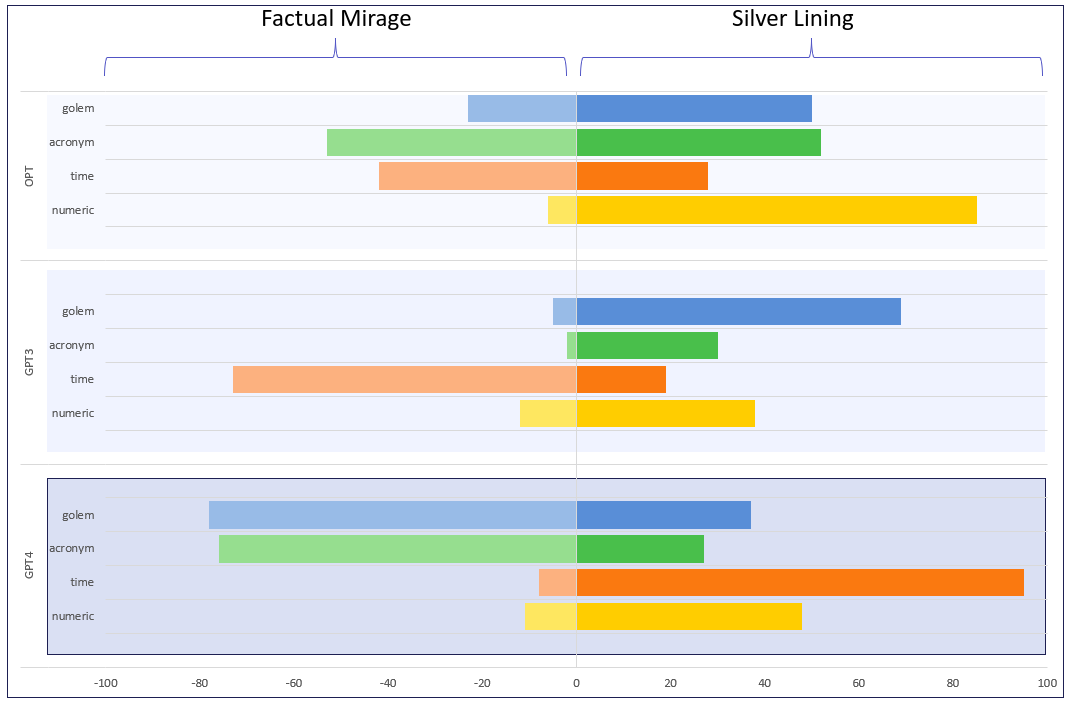
\includegraphics[width=\textwidth,height=9cm]{img/hvi.png}
    \caption{Hallucination Vulnerability Index \emph{(HVI)} for different hallucination categories for various LLMs \textcolor{red}{why does this figure have an arxiv link?}}
    \label{fig:hvi}
\end{figure}
% \qquad
% %\begin{table}[!ht]
%\tiny
%\centering
%\resizebox{0.32\textheight}{!}{%
\resizebox{0.9\columnwidth}{!}{%
\begin{tabular}{lll}
\toprule
\textbf{LLM} & \textbf{Size} & \textbf{HVI (0-100)}
\\ \midrule
\textbf{GPT-3}    &  175B       &   90 - 
\begin{tikzpicture}
\centering
\draw[red, very thick, fill=red] (0,0)  rectangle (5.62,.1);
\end{tikzpicture}
\\
\textbf{StableLM}    &  7B   &     82 - 
\begin{tikzpicture}
\centering
\draw[red, very thick, fill=red] (0,0)  rectangle (5.12,.1);
\end{tikzpicture}
\\
\textbf{GPT-2}    &   1.5B      &     70 - 
\begin{tikzpicture}
\centering
\draw[red, very thick, fill=red] (0,0)  rectangle (4.38,.1);
\end{tikzpicture}
\\
\textbf{Vicuna}     & 13B      &   62 - 
\begin{tikzpicture}
\centering
\draw[orange, very thick, fill=orange] (0,0)  rectangle (3.88,.1);
\end{tikzpicture}  
\\
\textbf{MPT}    &  7B    &     59 - 
\begin{tikzpicture}
\centering
\draw[orange, very thick, fill=orange] (0,0)  rectangle (3.69,.1);
\end{tikzpicture}   
\\
\textbf{LLaMA}    &  65B    &     57 - 
\begin{tikzpicture}
\centering
\draw[orange, very thick, fill=orange] (0,0)  rectangle (3.56,.1);
\end{tikzpicture}   
\\
\textbf{GPT-3.5}   &    175B      &     53 - 
\begin{tikzpicture}
\centering
\draw[orange, very thick, fill=orange] (0,0)  rectangle (3.31,.1);
\end{tikzpicture}
\\
\textbf{Dolly}    &   12B    &    49 - 
\begin{tikzpicture}
\centering
\draw[violet, very thick, fill=violet] (0,0)  rectangle (3.06,.1);
\end{tikzpicture} 
\\
\textbf{OPT}    &   175B   &     48 - \begin{tikzpicture}
\centering
\draw[violet, very thick, fill=violet] (0,0)  rectangle (3,.1);
\end{tikzpicture}   
\\
\textbf{GPT-4}    &   1.7T    &      47 - \begin{tikzpicture}
\centering
\draw[violet, very thick, fill=violet] (0,0)  rectangle (2.94,.1);
\end{tikzpicture}  
\\
\textbf{Alpaca}   &   65B    &     40 - \begin{tikzpicture}
\centering
\draw[violet, very thick, fill=violet] (0,0)  rectangle (2.5,.1);
\end{tikzpicture}   
\\
\textbf{BLOOM}   &   176B     &   38 - \begin{tikzpicture}
\centering
\draw[blue, very thick, fill=blue] (0,0)  rectangle (2.38,.1);
\end{tikzpicture}  
\\
\textbf{T0}    &      11B    &     36 - \begin{tikzpicture}
\centering
\draw[blue, very thick, fill=blue] (0,0)  rectangle (2.25,.1);
\end{tikzpicture}  
\\
\textbf{XLNet}   &   340M     &      36 - \begin{tikzpicture}
\centering
\draw[blue, very thick, fill=blue] (0,0)  rectangle (2.25,.1);
\end{tikzpicture}  
\\
\textbf{T5}    &    11B      &     32 - \begin{tikzpicture}
\centering
\draw[blue, very thick, fill=blue] (0,0)  rectangle (2.0,.1);
\end{tikzpicture}  
\\
% ERNIE           &     40 - \begin{tikzpicture}
% \centering
% \draw[violet, very thick, fill=violet] (0,0)  rectangle (2,.5);
% \end{tikzpicture}  
% \\
% ALBERT          &   33 - \begin{tikzpicture}
% \centering
% \draw[blue, very thick, fill=blue] (0,0)  rectangle (1.8,.5);
% \end{tikzpicture}    
% \\
% DeBERTa         &     32 - \begin{tikzpicture}
% \centering
% \draw[blue, very thick, fill=blue] (0,0)  rectangle (1.6,.5);
% \end{tikzpicture}    
% \\
% ELECTRA         &    32 - \begin{tikzpicture}
% \centering
% \draw[blue, very thick, fill=blue] (0,0)  rectangle (1.8,.5);
% \end{tikzpicture}     
% \\
% RoBERTa         &    28 - \begin{tikzpicture}
% \centering
% \draw[blue, very thick, fill=blue] (0,0)  rectangle (1.4,.5);
% \end{tikzpicture}     
% \\
% BERT            &    26 - \begin{tikzpicture}
% \centering
% \draw[blue, very thick, fill=blue] (0,0)  rectangle (1,.5);
% \end{tikzpicture}     
% \ \ 
\bottomrule
\end{tabular}%
}
%%
%}


%\caption{A ranked list of LLMs based on HVI.}
%\label{tab:LLMs}
%\end{table}
%\vspace{-3mm}









\begin{comment}
%\begin{table}[!ht]
%\tiny
%\centering
\resizebox{\columnwidth}{!}{%
\begin{tabular}{lll}
\toprule
\textbf{LLM} & \textbf{Size} & \textbf{HVI (0-100)}
\\ \midrule
\textbf{GPT 4}    &  N/A       &   90 - \begin{tikzpicture}
\centering
\draw[red, very thick, fill=red] (0,0)  rectangle (5,.1);
\end{tikzpicture}
\\
\textbf{GPT 3.5}    &  1.3B   &     82 - \begin{tikzpicture}
\centering
\draw[red, very thick, fill=red] (0,0)  rectangle (4.6,.1);
\end{tikzpicture}
\\
\textbf{GPT 3}     & 175B      &   70 - \begin{tikzpicture}
\centering
\draw[red, very thick, fill=red] (0,0)  rectangle (4.4,.1);
\end{tikzpicture}  
\\
\textbf{GPT 2}    &   1.5B    &      47 - \begin{tikzpicture}
\centering
\draw[red, very thick, fill=red] (0,0)  rectangle (4.2,.1);
\end{tikzpicture}  
\\
\textbf{MPT}   &    7B      &     59 - \begin{tikzpicture}
\centering
\draw[orange, very thick, fill=orange] (0,0)  rectangle (4.0,.1);
\end{tikzpicture}
\\
\textbf{OPT}    &   125M      &     59 - \begin{tikzpicture}
\centering
\draw[orange, very thick, fill=orange] (0,0)  rectangle (3.8,.1);
\end{tikzpicture}
\\
\textbf{LLaMA}    &   7B    &    52 - \begin{tikzpicture}
\centering
\draw[orange, very thick, fill=orange] (0,0)  rectangle (3.5,.1);
\end{tikzpicture} 
\\
\textbf{BLOOM}   &   175B     &   49 - \begin{tikzpicture}
\centering
\draw[orange, very thick, fill=orange] (0,0)  rectangle (3.3,.1);
\end{tikzpicture}  
\\
\textbf{Alpaca}    &   7B   &     44 - \begin{tikzpicture}
\centering
\draw[orange, very thick, fill=orange] (0,0)  rectangle (3.1,.1);
\end{tikzpicture}   
\\
\textbf{Vicuna}    &  7B    &     44 - \begin{tikzpicture}
\centering
\draw[violet, very thick, fill=violet] (0,0)  rectangle (2.9,.1);
\end{tikzpicture}   
\\
\textbf{Dolly}   &   12B    &     44 - \begin{tikzpicture}
\centering
\draw[violet, very thick, fill=violet] (0,0)  rectangle (2.7,.1);
\end{tikzpicture}   
\\
\textbf{StableLM}    &  3B    &     44 - \begin{tikzpicture}
\centering
\draw[violet, very thick, fill=violet] (0,0)  rectangle (2.5,.1);
\end{tikzpicture}   
\\
\textbf{XLNet}   &   110M     &      42 - \begin{tikzpicture}
\centering
\draw[blue, very thick, fill=blue] (0,0)  rectangle (2.3,.1);
\end{tikzpicture}  
\\
\textbf{T0}    &      11B    &     42 - \begin{tikzpicture}
\centering
\draw[blue, very thick, fill=blue] (0,0)  rectangle (2.2,.1);
\end{tikzpicture}  
\\
\textbf{T5}    &    3B      &     41 - \begin{tikzpicture}
\centering
\draw[blue, very thick, fill=blue] (0,0)  rectangle (2.0,.1);
\end{tikzpicture}  
\\
% ERNIE           &     40 - \begin{tikzpicture}
% \centering
% \draw[violet, very thick, fill=violet] (0,0)  rectangle (2,.5);
% \end{tikzpicture}  
% \\
% ALBERT          &   33 - \begin{tikzpicture}
% \centering
% \draw[blue, very thick, fill=blue] (0,0)  rectangle (1.8,.5);
% \end{tikzpicture}    
% \\
% DeBERTa         &     32 - \begin{tikzpicture}
% \centering
% \draw[blue, very thick, fill=blue] (0,0)  rectangle (1.6,.5);
% \end{tikzpicture}    
% \\
% ELECTRA         &    32 - \begin{tikzpicture}
% \centering
% \draw[blue, very thick, fill=blue] (0,0)  rectangle (1.8,.5);
% \end{tikzpicture}     
% \\
% RoBERTa         &    28 - \begin{tikzpicture}
% \centering
% \draw[blue, very thick, fill=blue] (0,0)  rectangle (1.4,.5);
% \end{tikzpicture}     
% \\
% BERT            &    26 - \begin{tikzpicture}
% \centering
% \draw[blue, very thick, fill=blue] (0,0)  rectangle (1,.5);
% \end{tikzpicture}     
% \\ 
\bottomrule
\end{tabular}%
}
%\caption{A ranked list of LLMs based on HVI.}
%\label{tab:LLMs}
%\end{table}
%\vspace{-3mm}
\end{comment}    
% \begin{tabular}[b]{cc}\hline
%   Table head & Table head \\ \hline
%   Some values & Some values \\
%   Some values & Some values \\
%   Some values & Some values \\
%   Some values & Some values \\
%   Some values & Some values \\
%   Some values & Some values \\ \hline
% \end{tabular}
% \captionlistentry[table]{A table beside a figure}
% \captionsetup{labelformat=andtable}
% \caption{A table beside a figure}
% \end{figure*}

% \begin{minipage}{0.35\linewidth}
% 		% \caption{Caption }
% 		\label{tab:le}
% 		\centering
%   %\begin{table}[!ht]
%\tiny
%\centering
%\resizebox{0.32\textheight}{!}{%
\resizebox{0.9\columnwidth}{!}{%
\begin{tabular}{lll}
\toprule
\textbf{LLM} & \textbf{Size} & \textbf{HVI (0-100)}
\\ \midrule
\textbf{GPT-3}    &  175B       &   90 - \begin{tikzpicture}
\centering
\draw[red, very thick, fill=red] (0,0)  rectangle (5.62,.1);
\end{tikzpicture}
\\
\textbf{StableLM}    &  7B   &     82 - \begin{tikzpicture}
\centering
\draw[red, very thick, fill=red] (0,0)  rectangle (5.12,.1);
\end{tikzpicture}
\\
\textbf{GPT-2}    &   1.5B      &     70 - \begin{tikzpicture}
\centering
\draw[red, very thick, fill=red] (0,0)  rectangle (4.38,.1);
\end{tikzpicture}
\\
\textbf{Vicuna}     & 13B      &   62 - \begin{tikzpicture}
\centering
\draw[orange, very thick, fill=orange] (0,0)  rectangle (3.88,.1);
\end{tikzpicture}  
\\
\textbf{MPT}    &  7B    &     59 - \begin{tikzpicture}
\centering
\draw[orange, very thick, fill=orange] (0,0)  rectangle (3.69,.1);
\end{tikzpicture}   
\\
\textbf{LLaMA}    &  65B    &     57 - \begin{tikzpicture}
\centering
\draw[orange, very thick, fill=orange] (0,0)  rectangle (3.56,.1);
\end{tikzpicture}   
\\
\textbf{GPT-3.5}   &    175B      &     53 - \begin{tikzpicture}
\centering
\draw[orange, very thick, fill=orange] (0,0)  rectangle (3.31,.1);
\end{tikzpicture}
\\
\textbf{Dolly}    &   12B    &    49 - \begin{tikzpicture}
\centering
\draw[violet, very thick, fill=violet] (0,0)  rectangle (3.06,.1);
\end{tikzpicture} 
\\
\textbf{OPT}    &   175B   &     48 - \begin{tikzpicture}
\centering
\draw[violet, very thick, fill=violet] (0,0)  rectangle (3,.1);
\end{tikzpicture}   
\\
\textbf{GPT-4}    &   1.7T    &      47 - \begin{tikzpicture}
\centering
\draw[violet, very thick, fill=violet] (0,0)  rectangle (2.94,.1);
\end{tikzpicture}  
\\
\textbf{Alpaca}   &   65B    &     40 - \begin{tikzpicture}
\centering
\draw[violet, very thick, fill=violet] (0,0)  rectangle (2.5,.1);
\end{tikzpicture}   
\\
\textbf{BLOOM}   &   176B     &   38 - \begin{tikzpicture}
\centering
\draw[blue, very thick, fill=blue] (0,0)  rectangle (2.38,.1);
\end{tikzpicture}  
\\
\textbf{T0}    &      11B    &     36 - \begin{tikzpicture}
\centering
\draw[blue, very thick, fill=blue] (0,0)  rectangle (2.25,.1);
\end{tikzpicture}  
\\
\textbf{XLNet}   &   340M     &      36 - \begin{tikzpicture}
\centering
\draw[blue, very thick, fill=blue] (0,0)  rectangle (2.25,.1);
\end{tikzpicture}  
\\
\textbf{T5}    &    11B      &     32 - \begin{tikzpicture}
\centering
\draw[blue, very thick, fill=blue] (0,0)  rectangle (2.0,.1);
\end{tikzpicture}  
\\
% ERNIE           &     40 - \begin{tikzpicture}
% \centering
% \draw[violet, very thick, fill=violet] (0,0)  rectangle (2,.5);
% \end{tikzpicture}  
% \\
% ALBERT          &   33 - \begin{tikzpicture}
% \centering
% \draw[blue, very thick, fill=blue] (0,0)  rectangle (1.8,.5);
% \end{tikzpicture}    
% \\
% DeBERTa         &     32 - \begin{tikzpicture}
% \centering
% \draw[blue, very thick, fill=blue] (0,0)  rectangle (1.6,.5);
% \end{tikzpicture}    
% \\
% ELECTRA         &    32 - \begin{tikzpicture}
% \centering
% \draw[blue, very thick, fill=blue] (0,0)  rectangle (1.8,.5);
% \end{tikzpicture}     
% \\
% RoBERTa         &    28 - \begin{tikzpicture}
% \centering
% \draw[blue, very thick, fill=blue] (0,0)  rectangle (1.4,.5);
% \end{tikzpicture}     
% \\
% BERT            &    26 - \begin{tikzpicture}
% \centering
% \draw[blue, very thick, fill=blue] (0,0)  rectangle (1,.5);
% \end{tikzpicture}     
% \ \ 
\bottomrule
\end{tabular}%
}
%%
%}


%\caption{A ranked list of LLMs based on HVI.}
%\label{tab:LLMs}
%\end{table}
%\vspace{-3mm}









\begin{comment}
%\begin{table}[!ht]
%\tiny
%\centering
\resizebox{\columnwidth}{!}{%
\begin{tabular}{lll}
\toprule
\textbf{LLM} & \textbf{Size} & \textbf{HVI (0-100)}
\\ \midrule
\textbf{GPT 4}    &  N/A       &   90 - \begin{tikzpicture}
\centering
\draw[red, very thick, fill=red] (0,0)  rectangle (5,.1);
\end{tikzpicture}
\\
\textbf{GPT 3.5}    &  1.3B   &     82 - \begin{tikzpicture}
\centering
\draw[red, very thick, fill=red] (0,0)  rectangle (4.6,.1);
\end{tikzpicture}
\\
\textbf{GPT 3}     & 175B      &   70 - \begin{tikzpicture}
\centering
\draw[red, very thick, fill=red] (0,0)  rectangle (4.4,.1);
\end{tikzpicture}  
\\
\textbf{GPT 2}    &   1.5B    &      47 - \begin{tikzpicture}
\centering
\draw[red, very thick, fill=red] (0,0)  rectangle (4.2,.1);
\end{tikzpicture}  
\\
\textbf{MPT}   &    7B      &     59 - \begin{tikzpicture}
\centering
\draw[orange, very thick, fill=orange] (0,0)  rectangle (4.0,.1);
\end{tikzpicture}
\\
\textbf{OPT}    &   125M      &     59 - \begin{tikzpicture}
\centering
\draw[orange, very thick, fill=orange] (0,0)  rectangle (3.8,.1);
\end{tikzpicture}
\\
\textbf{LLaMA}    &   7B    &    52 - \begin{tikzpicture}
\centering
\draw[orange, very thick, fill=orange] (0,0)  rectangle (3.5,.1);
\end{tikzpicture} 
\\
\textbf{BLOOM}   &   175B     &   49 - \begin{tikzpicture}
\centering
\draw[orange, very thick, fill=orange] (0,0)  rectangle (3.3,.1);
\end{tikzpicture}  
\\
\textbf{Alpaca}    &   7B   &     44 - \begin{tikzpicture}
\centering
\draw[orange, very thick, fill=orange] (0,0)  rectangle (3.1,.1);
\end{tikzpicture}   
\\
\textbf{Vicuna}    &  7B    &     44 - \begin{tikzpicture}
\centering
\draw[violet, very thick, fill=violet] (0,0)  rectangle (2.9,.1);
\end{tikzpicture}   
\\
\textbf{Dolly}   &   12B    &     44 - \begin{tikzpicture}
\centering
\draw[violet, very thick, fill=violet] (0,0)  rectangle (2.7,.1);
\end{tikzpicture}   
\\
\textbf{StableLM}    &  3B    &     44 - \begin{tikzpicture}
\centering
\draw[violet, very thick, fill=violet] (0,0)  rectangle (2.5,.1);
\end{tikzpicture}   
\\
\textbf{XLNet}   &   110M     &      42 - \begin{tikzpicture}
\centering
\draw[blue, very thick, fill=blue] (0,0)  rectangle (2.3,.1);
\end{tikzpicture}  
\\
\textbf{T0}    &      11B    &     42 - \begin{tikzpicture}
\centering
\draw[blue, very thick, fill=blue] (0,0)  rectangle (2.2,.1);
\end{tikzpicture}  
\\
\textbf{T5}    &    3B      &     41 - \begin{tikzpicture}
\centering
\draw[blue, very thick, fill=blue] (0,0)  rectangle (2.0,.1);
\end{tikzpicture}  
\\
% ERNIE           &     40 - \begin{tikzpicture}
% \centering
% \draw[violet, very thick, fill=violet] (0,0)  rectangle (2,.5);
% \end{tikzpicture}  
% \\
% ALBERT          &   33 - \begin{tikzpicture}
% \centering
% \draw[blue, very thick, fill=blue] (0,0)  rectangle (1.8,.5);
% \end{tikzpicture}    
% \\
% DeBERTa         &     32 - \begin{tikzpicture}
% \centering
% \draw[blue, very thick, fill=blue] (0,0)  rectangle (1.6,.5);
% \end{tikzpicture}    
% \\
% ELECTRA         &    32 - \begin{tikzpicture}
% \centering
% \draw[blue, very thick, fill=blue] (0,0)  rectangle (1.8,.5);
% \end{tikzpicture}     
% \\
% RoBERTa         &    28 - \begin{tikzpicture}
% \centering
% \draw[blue, very thick, fill=blue] (0,0)  rectangle (1.4,.5);
% \end{tikzpicture}     
% \\
% BERT            &    26 - \begin{tikzpicture}
% \centering
% \draw[blue, very thick, fill=blue] (0,0)  rectangle (1,.5);
% \end{tikzpicture}     
% \\ 
\bottomrule
\end{tabular}%
}
%\caption{A ranked list of LLMs based on HVI.}
%\label{tab:LLMs}
%\end{table}
%\vspace{-3mm}
\end{comment}    
% 		% \resizebox{\textwidth}{!}{%
% 		% \begin{tabular}[width=\linewidth]{@{}lll@{}}
%   %   \toprule
%   %   \textbf{Student} & \textbf{week} & \textbf{grade} \\ 
%   %   \midrule
%   %   Ada Lovelace & 2 & A \\
% 		% 	Linus Thorvalds & 8 & A \\
% 		% 	Bruce Willis & 12 & F \\
% 		% 	Richard Stallman & 10 & B \\
% 		% 	Grace Hopper & 12 & A \\
% 		% 	Alan Turing & 8 & C \\
% 		% 	Bill Gates & 6 & D \\
% 		% 	Steve Jobs & 4 & E \\
%   %   \bottomrule
%   %   \end{tabular}}
% 	\end{minipage}
%  % \hfill
% 	\begin{minipage}{0.6\linewidth}
% 		\centering
% 		% \captionof{figure}{Caption_2}
% 		\label{figu:re}
% 		\begin{figure}
% [!htbp]
    \centering
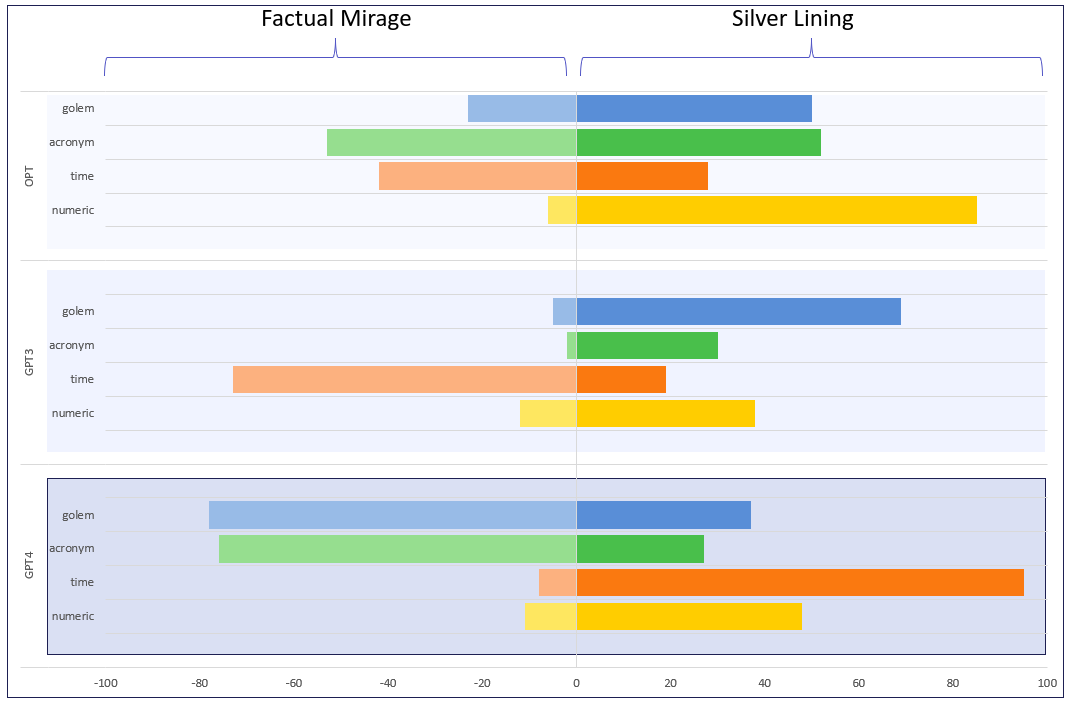
\includegraphics[width=\textwidth,height=9cm]{img/hvi.png}
    \caption{Hallucination Vulnerability Index \emph{(HVI)} for different hallucination categories for various LLMs \textcolor{red}{why does this figure have an arxiv link?}}
    \label{fig:hvi}
\end{figure}
%   % \includegraphics[width=0.8\textwidth]{Figs/Pair1.PNG}
% 	\end{minipage}

% \begin{table*}[!ht]%[H]
% \resizebox{0.98\textwidth}{!}{%
% \begin{tabular}{p{0.06\textwidth} | p{1.5\textwidth}} %{ll}
% \centering
% \toprule
% {\footnotesize \textbf{Prompt}} 
% & 
% \toprule
% \begin{footnotesize}
% \textit{USA's stance on Ukraine Russia war}
% \end{footnotesize}
% \\ \hline
% \rotatebox[origin=r]{90}{\parbox[c]{2cm}{\centering {\footnotesize \textbf{Hallucinated text}}}}
% & 
% \begin{footnotesize}
% {The official stance of the United States on the Russia-Ukraine war has been consistent in supporting Ukraine's sovereignty, territorial integrity, and the peaceful resolution of the conflict. The U.S. has condemned Russia's actions in annexing Crimea and its support for separatist movements in eastern Ukraine. Despite maintaining a diplomatic stance,  \colorbox{pink}{the U.S. President Barack Obama} stated that the United States would not deploy troops to Ukraine. Additionally, this lack of support extends to the withholding of financial and military assistance, including military equipment, training, and advisory support. This \colorbox{pink}{sentiment was reiterated} by \colorbox{pink}{Paul Altman} during a press review at the White House...}
% \end{footnotesize}
% \\ \hline
% \rotatebox[origin=r]{90}{\parbox[c]{2cm}{\centering {\footnotesize \textbf{Mitigated text\\\textcolor{blue}{ENTROPY\textsubscript{BB}}}}}}
% & 
% \begin{footnotesize}
% The official stance of the \colorbox{violet}{\textcolor{white}{government}} on the \colorbox{violet}{\textcolor{white}{ongoing}} war has been consistent in supporting \colorbox{violet}{\textcolor{white}{ resolution}} of the conflict. The \colorbox{violet}{\textcolor{white}{government}} has \colorbox{violet}{\textcolor{white}{condemned Russia}} in \colorbox{violet}{\textcolor{white}{country}} and its support for separatist movements in eastern \colorbox{violet}{\textcolor{white}{Ukraine}}. Despite maintaining a \colorbox{violet}{\textcolor{white}{neutral}} stance, the \colorbox{violet}{\textcolor{white}{government}} stated that the \colorbox{violet}{\textcolor{white}{country}} would not deploy troops to \colorbox{violet}{\textcolor{white}{unknown}}. Additionally, this lack of support extends to the withholding of financial and \colorbox{violet}{\textcolor{white}{resources}}, including \colorbox{violet}{\textcolor{white}{administrative}}, \colorbox{violet}{\textcolor{white}{technical}}, and \colorbox{violet}{\textcolor{white}{legal}}. This sentiment was \colorbox{violet}{\textcolor{white}{echoed}} by \colorbox{violet}{\textcolor{white}{minister}} during a press review at the \colorbox{violet}{\textcolor{white}{conference}}...
% \end{footnotesize}
% \\ \hline
% \rotatebox[origin=r]{90}{\parbox[c]{2.5cm}{\centering {\footnotesize \textbf{Edit Suggestions\\\textcolor{blue}{FACTUALITY\textsubscript{GB}}}}}}
% & 
% \begin{footnotesize}
% The official stance of the United States on the Russia-Ukraine war has been consistent in supporting Ukraine's sovereignty, territorial integrity, and the peaceful resolution of the conflict. The U.S. has condemned Russia's actions in annexing Crimea and its support for separatist movements in eastern Ukraine. \colorbox{red}{\textcolor{white}{Despite maintaining a diplomatic stance, the U.S. President Barack Obama stated that the United States would not deploy troops to Ukraine.}}\colorbox{orange}{\textcolor{white}{Additionally, this lack of support extends to t-}} \colorbox{orange}{\textcolor{white}{he withholding of financial and military assistance, including military equipment, training, and advisory support.}} \colorbox{red}{\textcolor{white}{This sentiment was reiterated by Paul Altman during a press review at th-}} \colorbox{red}{\textcolor{white}{e White House}}...
% \end{footnotesize}
% \\ \bottomrule
% \end{tabular}%
% }
% \caption{A hallucination example pre- and post-mitigation using an NYT tweet as a prompt. (Top) An output sample from an LLM that involves hallucinated components; (Bottom) A "mitigated" sample that shows a reduction in hallucination.}
% \label{tab:hallucination_ex}
% %\acil{I recommend replacing this example with an example that has a factual hallucination. Reviewers may argue that the impact of replacing the detected HE words is inconsequential -- it does not significantly change the perception of the story.}
% \end{table*}